\documentclass[11pt,a4paper,english]{article}
% Adapted from the user's Rapportmal UiA. Compile with pdfLaTeX on Overleaf.
\usepackage[T1]{fontenc}
\usepackage[utf8]{inputenc}
\usepackage{babel}
\usepackage{lmodern,microtype}
\usepackage[a4paper,margin=25mm,headheight=15pt]{geometry}
\usepackage{amsmath,amssymb,mathtools}
\usepackage{graphicx,svg}
\usepackage{booktabs,tabularx,array}
\usepackage[font=small,labelfont=bf]{caption}
\usepackage{float,placeins}
\usepackage{parskip}
\usepackage{xcolor,fancyhdr}
\usepackage{enumitem}
\usepackage{listings}
\usepackage[hidelinks]{hyperref}
\usepackage[nameinlink,noabbrev]{cleveref}
\definecolor{uiaaccent}{HTML}{185E68}
\pagestyle{fancy}
\fancyhf{}
\fancyhead[L]{\small MA-447 \enspace AI Mathematics}
\fancyhead[R]{\small PCA and eigenfaces}
\fancyfoot[C]{\thepage}
\renewcommand{\headrulewidth}{0.3pt}
\setlength{\parskip}{5pt plus 1pt}
\setlength{\emergencystretch}{2em}
\setlist{itemsep=2pt,topsep=4pt}
\setcounter{tocdepth}{1}
\numberwithin{equation}{section}
\DeclareMathOperator{\tr}{tr}
\DeclareMathOperator{\rank}{rank}
\DeclareMathOperator*{\argmin}{arg\,min}
\newcommand{\R}{\mathbb{R}}
\newcommand{\norm}[1]{\left\lVert#1\right\rVert}
\newcommand{\T}{^{\mathsf T}}
\hypersetup{pdftitle={Principal Component Analysis for Image Recognition},pdfauthor={Kristian Eieland}}
\lstset{basicstyle=\ttfamily\footnotesize,breaklines=true,columns=fullflexible,keepspaces=true,showstringspaces=false}

\begin{document}
\begin{titlepage}
\centering
\vspace*{4mm}
\includesvg[width=.80\textwidth]{images/uia_logo_english}\par
\vspace{20mm}
{\color{uiaaccent}\LARGE\bfseries Principal Component Analysis\\[3mm] for Image Recognition\par}
\vspace{8mm}
{\large A mathematical analysis of Turk and Pentland's\\[2mm]\textit{Eigenfaces for Recognition}\par}
\vspace{17mm}
{\Large Kristian Eieland\par}
\vspace{8mm}
{\large MA-447: AI Mathematics\par}
\vspace{3mm}
Course assignment \textbullet\ Group 8: PCA\par
\vspace{13mm}

Faculty of Engineering and Science\\
University of Agder
\vfill
{\large 1 October 2026\par}
\vspace{8mm}
\end{titlepage}

\pagenumbering{roman}
\section*{Abstract}
\addcontentsline{toc}{section}{Abstract}
This report studies principal component analysis (PCA) in Turk and Pentland's eigenface method for image recognition. It derives the covariance eigenvalue problem from variance maximization and shows why the leading eigenvectors minimize squared reconstruction error. The smaller Gram matrix allows the same directions to be calculated when each image has more pixels than there are training images. A four point example gives the calculations explicitly. In a separate experiment on handwritten digits, validation accuracy selects 30 of 64 components. A nearest-centroid classifier then correctly labels 316 of 360 test images, the same count as a classifier using all 64 pixels. PCA therefore reduces the number of coordinates in this experiment without changing the observed test accuracy. The digit experiment illustrates the method. It does not reproduce the paper's face recognition results.
\vspace{5mm}
\tableofcontents
\clearpage
\pagenumbering{arabic}

\section{Selected paper and scope}
The selected research article is Matthew Turk and Alex Pentland, \emph{Eigenfaces for Recognition}, published in the \emph{Journal of Cognitive Neuroscience}, 3(1), 71--86, in 1991 \cite{turk}. Its application is face recognition. Each centered face image is represented by weights on a small set of covariance eigenvectors, called eigenfaces. Recognition compares these weights with representations of known people; a reconstruction residual helps distinguish images outside the learned face subspace.

The analysis follows the variance-maximization problem and the smaller eigenproblem in the paper's ``Calculating Eigenfaces'' section, especially Eqs.~(1)--(6), pp.~74--75. This report stores images in rows, while the paper stores centered images in columns. Eigenfaces describe variation across whole images and need not correspond to individual features such as eyes or noses.

The derivation explains why maximizing retained variance selects covariance eigenvectors and how their projection weights can be used for recognition. The supplementary experiment applies the calculation to handwritten digits. Face-recognition performance would require a separate experiment with face images.

\section{Data representation and notation}
An image is flattened into a column vector $x_i\in\R^p$. The coordinates refer to corresponding pixel locations across images. Flattening rearranges the values without changing them. The data matrix $X\in\R^{n\times p}$ stores $x_i\T$ in row $i$.

\begin{table}[htbp]
\centering
\caption{Notation. The mean and PCA directions are learned from the fitting data only.}
\label{tab:notation}
\begin{tabularx}{\textwidth}{@{}l l X@{}}
\toprule Symbol & Shape & Meaning \\
\midrule
$X$ & $n\times p$ & Observations in rows \\
$\mu$ & $p\times1$ & Mean image or mean observation \\
$X_c$ & $n\times p$ & Centered observations \\
$S$ & $p\times p$ & Sample covariance matrix \\
$u_j,\lambda_j$ & $p\times1$, scalar & Principal direction and its score variance \\
$U_k$ & $p\times k$ & First $k$ orthonormal principal directions \\
$Z$ & $n\times k$ & Reduced coordinates, also called scores \\
\bottomrule
\end{tabularx}
\end{table}

For $n\geq2$, define the mean and centered matrix by
\begin{equation}
\mu=\frac1n\sum_{i=1}^{n}x_i,
\qquad X_c=X-\mathbf1_n\mu\T.
\label{eq:center}
\end{equation}
The sample covariance is
\begin{equation}
S=\frac{1}{n-1}X_c\T X_c
=\frac{1}{n-1}\sum_{i=1}^n(x_i-\mu)(x_i-\mu)\T.
\label{eq:cov}
\end{equation}
Its diagonal entries are feature variances; its off-diagonal entries describe how pairs of features vary together. It is symmetric and positive semidefinite because
$v\T Sv=\norm{X_cv}_2^2/(n-1)\geq0$ for every $v$.

The article's column matrix $A$ corresponds to $X_c\T$. Its average-variance convention uses $1/n$, whereas this report uses $1/(n-1)$. For unscaled centered columns, $AA\T$ is the scatter matrix. Either positive normalizing factor changes the eigenvalues while preserving their order, eigenvectors and explained-variance ratios. The factor must therefore be included when comparing eigenvalues from the two conventions.

\section{Why PCA is an eigenvalue problem}
\subsection{Variance maximization}
Let $u\in\R^p$ be a unit vector. Projecting image $i$ onto this direction gives the scalar $z_i=u\T(x_i-\mu)$. These scores have mean zero, so their sample variance is
\begin{equation}
\operatorname{Var}(z)=\frac1{n-1}\sum_{i=1}^n\bigl(u\T(x_i-\mu)\bigr)^2
=u\T Su.
\label{eq:variance}
\end{equation}
The first principal direction therefore solves
\begin{equation}
\max_{u\in\R^p} u\T Su
\quad\text{subject to}\quad u\T u=1.
\label{eq:objective}
\end{equation}
The unit-length constraint fixes the scale. Without it, multiplying a direction with positive variance by an arbitrarily large constant would make the objective unbounded. This is the standard variance formulation of PCA \cite{jolliffe}.

\subsection{Stationary directions and the global maximum}
Introduce a Lagrange multiplier $\lambda$:
\begin{equation}
\mathcal L(u,\lambda)=u\T Su-\lambda(u\T u-1).
\end{equation}
Since $S=S\T$, differentiation yields
\begin{equation}
\nabla_u\mathcal L=2Su-2\lambda u=0
\quad\Longrightarrow\quad Su=\lambda u.
\label{eq:eigen}
\end{equation}
Thus every stationary direction is an eigenvector. This calculation alone does not prove which stationary direction is a maximum.

Because $S$ is real and symmetric, it has an orthonormal eigenbasis $q_1,\ldots,q_p$ with eigenvalues $\lambda_1\geq\cdots\geq\lambda_p\geq0$. Every unit vector can be written as $u=\sum_j a_jq_j$, with $\sum_j a_j^2=1$. Hence
\begin{equation}
u\T Su=\sum_{j=1}^p\lambda_j a_j^2
\leq\lambda_1\sum_{j=1}^p a_j^2=\lambda_1.
\label{eq:maximum}
\end{equation}
The upper bound is attained by $u=q_1$. The largest eigenvalue is therefore the maximum attainable score variance, and its eigenvector gives a maximizing direction. When the leading eigenvalue is repeated, any unit vector in its eigenspace is optimal. Changing the sign of a direction changes score signs but not the projection or reconstruction.

\subsection{Several components}
For $k$ directions, the constraint becomes $U\T U=I_k$, and the retained total variance is $\tr(U\T SU)$. In the eigenbasis,
\begin{equation}
\tr(U\T SU)=\sum_{j=1}^p\lambda_j w_j,
\qquad w_j=\norm{U\T q_j}_2^2,
\quad 0\leq w_j\leq1,\quad\sum_jw_j=k.
\end{equation}
No allocation of these weights can exceed $\lambda_1+\cdots+\lambda_k$: moving weight from a smaller eigenvalue to a larger one never decreases the sum. Choosing $U_k=[q_1\ \cdots\ q_k]$ attains this bound. A tie at the cutoff can make the optimal $k$-dimensional subspace non-unique.

\section{Projection, reconstruction and information loss}
\subsection{The reduced representation}
The matrix of scores and its sample covariance are
\begin{equation}
Z=X_cU_k,\qquad
\frac{Z\T Z}{n-1}=U_k\T SU_k
=\operatorname{diag}(\lambda_1,\ldots,\lambda_k).
\label{eq:scores}
\end{equation}
The score coordinates are uncorrelated on the fitting sample. Uncorrelated variables need not be statistically independent; no Gaussian assumption is needed to calculate PCA.

For a new image $x$, the fitted mean and directions remain fixed:
\begin{equation}
z=U_k\T(x-\mu),\qquad
\hat x=\mu+U_kz=\mu+U_kU_k\T(x-\mu).
\label{eq:reconstruct}
\end{equation}
The retained fraction of fitting-sample variance, provided $\tr(S)>0$, is
\begin{equation}
R_k=\frac{\sum_{j=1}^k\lambda_j}{\sum_{j=1}^p\lambda_j}.
\label{eq:ratio}
\end{equation}
This is a variance ratio, not a classification accuracy. When all $p$ orthonormal directions are retained, every observation can be reconstructed exactly, up to numerical error. Keeping only the nonzero fitting directions reconstructs the fitting data exactly, but need not reconstruct a new image outside their span.

\subsection{Why PCA minimizes squared reconstruction error}
Let $P=UU\T$, where $U\T U=I_k$. Then $P\T=P$ and $P^2=P$, so $P$ is an orthogonal projector. The squared Frobenius norm sums squared errors across all observations and features. Using the cyclic property of the trace,
\begin{align}
E(U)&=\norm{X_c-X_cP}_F^2\nonumber\\
&=\tr\bigl((I-P)X_c\T X_c(I-P)\bigr)\nonumber\\
&=\tr(X_c\T X_c)-\tr(U\T X_c\T X_cU)\nonumber\\
&=(n-1)\bigl[\tr(S)-\tr(U\T SU)\bigr].
\label{eq:errorproof}
\end{align}
The first term is fixed by the data. Minimizing reconstruction error is therefore equivalent to maximizing the retained variance. At the PCA optimum,
\begin{equation}
\boxed{\norm{X_c-X_cU_kU_k\T}_F^2=(n-1)\sum_{j=k+1}^p\lambda_j.}
\label{eq:discarded}
\end{equation}
The pixel mean squared error (MSE) on these same data divides this expression by $np$. The identity concerns the fitting data. Test MSE must be measured on the held-out observations and is not given by the discarded fitting eigenvalues.

For a fixed nested orthonormal basis, adding components cannot increase an observation's squared reconstruction error. That statement does not extend to classification accuracy: retaining an additional noisy direction can alter the nearest class in an unhelpful way.

\subsection{Rank and singular value decomposition}
The centered rows sum to zero, so
\begin{equation}
\rank(X_c)\leq\min(n-1,p).
\end{equation}
Only that many covariance eigenvalues can be positive. Write a reduced singular value decomposition as $X_c=Q\Sigma V\T$, using its nonzero singular values. Then
\begin{equation}
S=V\frac{\Sigma^2}{n-1}V\T,
\qquad \lambda_j=\frac{\sigma_j^2}{n-1}.
\label{eq:svd}
\end{equation}
The right singular vectors are the nonzero principal directions. Forming $X_c\T X_c$ squares the ratio of the largest to smallest nonzero singular values, which can amplify numerical conditioning problems. Direct SVD is therefore often preferable. The covariance calculation used here is checked against a full-SVD implementation \cite{sklearnpca}.

\section{From image geometry to recognition}
\subsection{The smaller eigenproblem}
When $p\gg n$, a $p\times p$ covariance matrix is expensive to store and decompose. Instead define the sample Gram matrix
\begin{equation}
G=\frac{X_cX_c\T}{n-1}\in\R^{n\times n},
\qquad Gv=\lambda v,\quad v\T v=1,\quad\lambda>0.
\label{eq:gram}
\end{equation}
Multiplication by $X_c\T$ gives
\begin{equation}
S(X_c\T v)
=X_c\T Gv=\lambda(X_c\T v).
\end{equation}
The mapped vector is thus an image-space eigenvector. Its length is not generally one:
\begin{equation}
\norm{X_c\T v}_2^2=v\T X_cX_c\T v=(n-1)\lambda.
\end{equation}
The normalized direction is consequently
\begin{equation}
u=\frac{X_c\T v}{\sqrt{(n-1)\lambda}}.
\label{eq:dualnormalize}
\end{equation}
Zero eigenvalues must be excluded from this formula. Under the same normalization, both constructions have the same nonzero eigenvalues. The Gram matrix requires storage of order $n^2$, compared with $p^2$ for the covariance matrix; the data and mapped directions also require storage. Turk and Pentland use this smaller matrix to calculate eigenfaces \cite[pp.~74--75]{turk}. It saves matrix storage when $n<p$. The digit experiment has only 64 features and uses the covariance matrix directly.

\subsection{PCA and the classification rule}
PCA learns directions without class labels. To make predictions, the supplementary experiment adds a nearest-centroid classifier. For each class $c$, let
\begin{equation}
m_c=\frac1{n_c}\sum_{i:y_i=c}z_i,
\qquad \hat y(x)=\argmin_c\norm{U_k\T(x-\mu)-m_c}_2^2.
\label{eq:classifier}
\end{equation}
Class labels are used to calculate the centroids. The classifier always assigns one of the ten known digit labels, with no threshold for rejecting an unknown class.

Projection also changes the distance between original observations:
\begin{equation}
\norm{U_k\T(x-y)}_2^2=(x-y)\T U_kU_k\T(x-y).
\label{eq:distance}
\end{equation}
Differences perpendicular to the retained subspace receive zero weight. Those differences may contain noise or features that distinguish classes. Centroid comparisons use $k$ coordinates after projection, but calculating each score vector requires a matrix--vector multiplication of order $pk$. Whether the complete classifier runs faster depends on both costs.

\subsection{Scaling and generalization}
In images, brightness or imperfect alignment may account for more variance than the differences between classes. A direction with little variance can still help distinguish two labels. This is why the experiment selects $k$ using classification accuracy on validation data.

Multiplying all pixels by one positive constant preserves PCA directions; scaling features separately can change them. Here the pixels share a common intensity range, so the experiment uses neither feature standardization nor whitening. The mean and PCA directions are fitted without test observations to keep test information out of model selection \cite{leakage}.

\section{A complete four-point calculation}
Consider $(5,4),(4,5),(2,1),(1,2)$. Their mean is $(3,3)$, and
\begin{equation}
X_c=\begin{pmatrix}2&1\\1&2\\-1&-2\\-2&-1\end{pmatrix},
\qquad S=\frac13\begin{pmatrix}10&8\\8&10\end{pmatrix}.
\end{equation}
The characteristic equation is
\begin{equation}
\det(S-\lambda I)=\left(\frac{10}3-\lambda\right)^2-\frac{64}9
=\lambda^2-\frac{20}3\lambda+4
=(\lambda-6)(\lambda-\tfrac23)=0.
\end{equation}
Thus $\lambda_1=6$, $\lambda_2=2/3$, with unit directions
\begin{equation}
u_1=\frac1{\sqrt2}\begin{pmatrix}1\\1\end{pmatrix},
\qquad u_2=\frac1{\sqrt2}\begin{pmatrix}1\\-1\end{pmatrix}.
\end{equation}
One component retains $6/(6+2/3)=0.90$, or 90\% of the variance. The first two scores are $3/\sqrt2$ and the last two are $-3/\sqrt2$. Reconstruction gives $(4.5,4.5)$ twice and $(1.5,1.5)$ twice. Each squared residual is $0.5$, so the total error is $2$. This agrees with \cref{eq:discarded}: $(n-1)\lambda_2=3(2/3)=2$.

\begin{figure}[htbp]
\centering
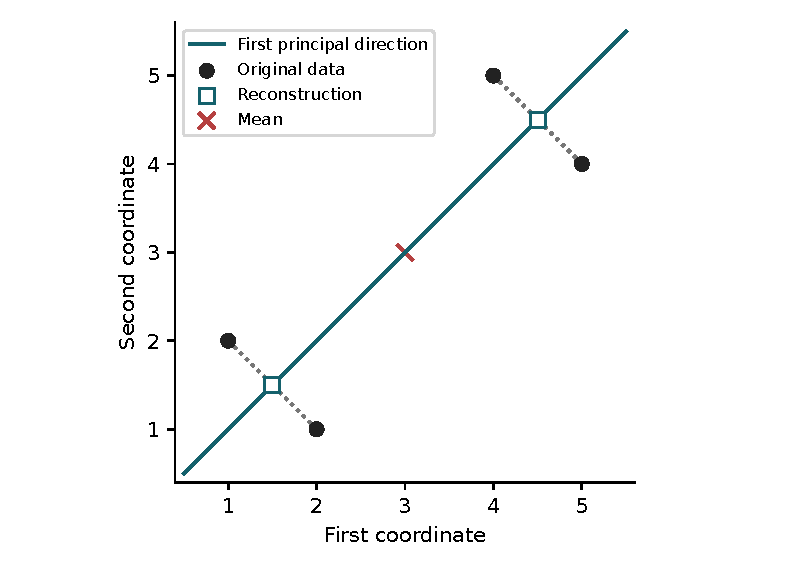
\includegraphics[width=.72\textwidth]{worked-example.pdf}
\caption{Projection of the four points onto the first principal direction. Dotted segments show the perpendicular residuals. Two points share each reconstructed location because their difference lies along the discarded direction.}
\label{fig:worked}
\end{figure}
\FloatBarrier

\section{Supplementary experiment on handwritten digits}
\subsection{Data and reproducible protocol}
The experiment uses scikit-learn's bundled \texttt{digits} dataset: 1,797 images from ten digit classes, with 64 pixel features per $8\times8$ image \cite{digits}. Pixel intensities range from 0 to 16 and are divided by 16. This fixed scaling does not estimate any dataset statistics. The split is stratified by digit label, not by writer, and differs from the original UCI benchmark protocol.

The data are split and processed as follows:
\begin{enumerate}
\item Split the indices into 1,437 development and 360 test observations. Use scikit-learn's \texttt{train\_test\_split} with \texttt{test\_size=0.2}, stratification by digit label, and random seed 42 (\texttt{random\_state=42}).
\item Split the development indices into 1,077 training and 360 validation observations with \texttt{test\_size=0.25}, stratification by their labels, and \texttt{random\_state=42} again.
\item Fit the mean, covariance eigenvectors and class centroids using training data only. Compare $k\in\{2,5,10,15,20,30,40,64\}$ on validation accuracy. Resolve ties by choosing the smallest $k$.
\item Refit the mean, PCA basis and class centroids on all 1,437 development observations, keeping the chosen $k$ fixed. Evaluate once on the held-out test observations, alongside a nearest-centroid baseline using all 64 original pixels.
\end{enumerate}
The test labels play no role in fitting or selecting $k$. The complete split indices and per-image test predictions are saved with the project.

\clearpage
\subsection{Validation results and choice of dimension}
\begin{table}[htbp]
\centering
\caption{Results before refitting: PCA is fitted to 1,077 training images, and prediction and reconstruction are evaluated on 360 validation images. MSE averages over images and pixels.}
\label{tab:validation}
\small
\begin{tabular}{@{}rrrrr@{}}
\toprule
$k$ & Variance retained (\%) & Correct / 360 & Accuracy (\%) & Pixel MSE \\
\midrule
2  & 28.50 & 221 & 61.39 & 0.052773 \\
5  & 54.84 & 291 & 80.83 & 0.034074 \\
10 & 74.07 & 314 & 87.22 & 0.019902 \\
15 & 83.68 & 321 & 89.17 & 0.012797 \\
20 & 89.65 & 324 & 90.00 & 0.008399 \\
\textbf{30} & \textbf{96.06} & \textbf{325} & \textbf{90.28} & \textbf{0.003381} \\
40 & 98.86 & 325 & 90.28 & 0.000991 \\
64 & 100.00 & 325 & 90.28 & $<10^{-28}$ \\
\bottomrule
\end{tabular}
\end{table}
With 30, 40 or 64 components, the classifier gives 325 correct validation predictions. The tie rule therefore selects $k=30$. Increasing $k$ from 30 to 40 lowers reconstruction MSE from 0.003381 to 0.000991, but leaves the number of correct predictions unchanged.

\subsection{Held-out test results}
After refitting, the 30 retained directions explain 95.94\% of development variance. This differs from the 96.06\% in \cref{tab:validation} because the covariance has been fitted to 1,437 rather than 1,077 observations.

\begin{table}[htbp]
\centering
\caption{Final comparison on the same 360 held-out images. Both classifiers use the same development observations.}
\label{tab:test}
\begin{tabular}{@{}lrr@{}}
\toprule & PCA + nearest centroid & Original-pixel baseline \\
\midrule
Coordinates per image & 30 & 64 \\
Correct predictions & 316 / 360 & 316 / 360 \\
Test accuracy & 87.78\% & 87.78\% \\
\bottomrule
\end{tabular}
\end{table}
The test reconstruction MSE is $0.0032097784$ on the normalized intensity scale. Using 30 instead of 64 coordinates is a reduction of 53.125\%, since $(64-30)/64=0.53125$. The mean and projection matrix require additional storage, so this percentage describes the coordinate count only. Both classifiers misclassify 44 test images. A single split does not show whether their accuracy would remain equal on other samples.

\begin{figure}[htbp]
\centering
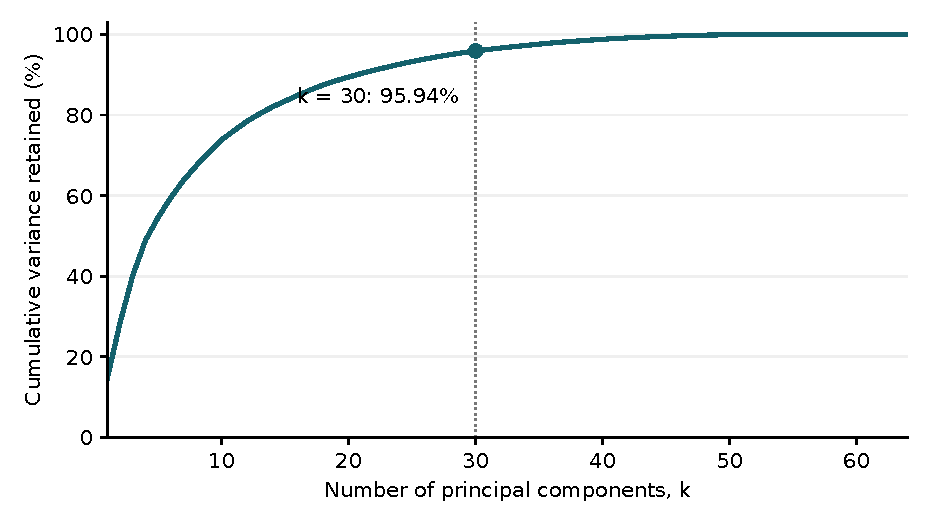
\includegraphics[width=.86\textwidth]{retained-variance.pdf}
\caption{Cumulative variance for the final PCA fit on the 1,437 development images. The selected 30 directions retain 95.94\%. This curve describes the refitted representation; the choice of $k$ was made earlier using validation accuracy.}
\label{fig:variance}
\end{figure}
\FloatBarrier

\subsection{Visual and numerical verification}
\begin{figure}[htbp]
\centering
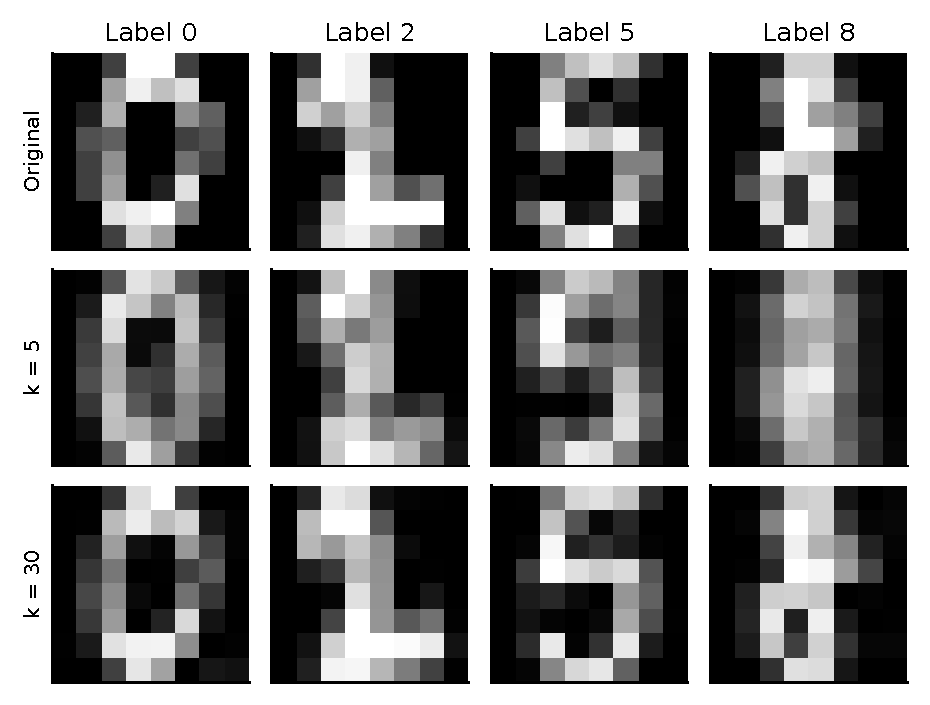
\includegraphics[width=.86\textwidth]{digit-reconstructions.pdf}
\caption{Four test digits reconstructed with 5 and 30 components of the development basis. Each column uses the first test observation with the indicated label in the saved split order. Images share a display range of $[0,1]$; error calculations use the unmodified reconstructed values.}
\label{fig:digits}
\end{figure}
The four-point example is verified against exact eigenvalues, reconstructions and total error. For the digit fit, the maximum absolute entry difference between the custom 30-component projector and scikit-learn's full-SVD projector is $3.22\times10^{-15}$. Projectors are compared because eigenvector signs are arbitrary. The measured development reconstruction sum of squares is $273.29359912095526$; the discarded-eigenvalue expression gives $273.2935991209546$, agreeing to floating-point precision.

The dual construction is checked separately on the first 32 training images ($n=32,p=64$). Its rank is 31, satisfying the centering bound. Its projector differs from the covariance projector by at most $8.25\times10^{-15}$ per entry. Keeping all 64 orthonormal directions also produces exactly the same predicted labels as the original-pixel classifier, as expected from preservation of Euclidean distances.
\FloatBarrier

\section{Conclusion}
The leading covariance eigenvectors maximize retained variance and minimize squared reconstruction error on centered fitting data. When images have more pixels than there are observations, the same nonzero directions can be calculated from the smaller Gram matrix. These directions form the eigenfaces used to represent images by a limited number of weights.

In the digit experiment, 30 components preserve 95.94\% of development variance and give 316 correct predictions out of 360 test images, matching the original-pixel baseline. For this split and classifier, the smaller representation preserves the observed accuracy. The reconstruction optimum follows from the derivation; classification performance still has to be measured on held-out data.

\clearpage
\phantomsection
\addcontentsline{toc}{section}{References}
\begin{thebibliography}{9}
\raggedright
\bibitem{turk} M. Turk and A. Pentland, ``Eigenfaces for Recognition,'' \emph{Journal of Cognitive Neuroscience}, vol.~3, no.~1, pp.~71--86, 1991. \href{https://doi.org/10.1162/jocn.1991.3.1.71}{doi:10.1162/jocn.1991.3.1.71}. Accessible copy: \url{https://courses.compute.dtu.dk/02503/docs/Eigenfaces1991.pdf}.
\bibitem{jolliffe} I. T. Jolliffe and J. Cadima, ``Principal component analysis: a review and recent developments,'' \emph{Philosophical Transactions of the Royal Society A}, vol.~374, no.~2065, art.~20150202, 2016. \href{https://doi.org/10.1098/rsta.2015.0202}{doi:10.1098/rsta.2015.0202}.
\bibitem{digits} Scikit-learn developers, ``load\_digits,'' \emph{Scikit-learn 1.7.2 documentation}. \url{https://scikit-learn.org/1.7/modules/generated/sklearn.datasets.load_digits.html}. Accessed 8 October 2026.
\bibitem{sklearnpca} Scikit-learn developers, ``PCA,'' \emph{Scikit-learn 1.7.2 documentation}. \url{https://scikit-learn.org/1.7/modules/generated/sklearn.decomposition.PCA.html}. Accessed 8 October 2026.
\bibitem{leakage} Scikit-learn developers, ``Common pitfalls and recommended practices: data leakage,'' \emph{Scikit-learn 1.7.2 documentation}. \url{https://scikit-learn.org/1.7/common_pitfalls.html\#data-leakage}. Accessed 8 October 2026.
\bibitem{lecture3} S. Rogovchenko, \emph{Analytic Geometry}, MA-447 lecture~3 slides, University of Agder, September 2026, pp.~13, 23, 33--39. \href{https://uia.instructure.com/courses/20940/files/3391641?wrap=1}{Course slides on Canvas}.
\bibitem{lecture4} S. Rogovchenko, \emph{Matrix Decompositions}, MA-447 lecture~4 slides, University of Agder, September 2026, pp.~16--17, 41, 58--59, 70--73. \href{https://uia.instructure.com/courses/20940/files/3402207?wrap=1}{Course slides on Canvas}.
\bibitem{lecture6} S. Rogovchenko, \emph{Continuous Optimization}, MA-447 lecture~6 slides, University of Agder, September 2026, pp.~26--32. \href{https://uia.instructure.com/courses/20940/files/3421696?wrap=1}{Course slides on Canvas}.
\end{thebibliography}

\appendix
\section{Reproducing the numerical checks}
The supplementary file \texttt{verify\_experiment.py} is a complete implementation. It loads the bundled digits dataset, saves the exact split indices and test predictions, generates all three figures, and writes \texttt{verified-results.json}. It requires NumPy, scikit-learn and Matplotlib. It does not download a separate image collection.

The code, result files and report source are available at\par
\url{https://github.com/KrisEie/ma447-pca-eigenfaces}.

\begin{lstlisting}
python -m pip install numpy==2.3.5 scikit-learn==1.7.2 matplotlib==3.11.2
python verify_experiment.py
\end{lstlisting}
The reported run used Python 3.12.14, NumPy 2.3.5, scikit-learn 1.7.2 and Matplotlib 3.11.2. The script checks that the splits are disjoint and verifies the worked example, covariance/SVD agreement, dual construction and reconstruction identity. It also checks that keeping all coordinates gives the same predictions as the baseline. Small floating-point differences across platforms are expected.
\clearpage
\section{Individual contribution and reflection}
\label{sec:individual}
\textbf{Kristian Eieland}

\subsection{Work completed for this report}
The report develops Turk and Pentland's PCA formulation using images stored as rows of a data matrix. It derives the variance-maximizing directions and reconstruction error, then shows how the smaller Gram matrix gives the same nonzero principal directions. The four-point example works through the mean, covariance, eigenvalues and reconstructed points, so each step can be checked by hand.

The Python experiment uses separate training, validation and test sets. It selects the number of components on validation accuracy and compares the resulting classifier with one using all pixels. The checks compare the covariance implementation with SVD and the dual construction, and compare measured reconstruction error with the sum of discarded eigenvalues. The figures show the projection in the worked example, cumulative variance and reconstructed digits.

\subsection{Why centering changes the calculation}
The centering step deserves a closer look because skipping it changes the matrix being decomposed. The covariance measures variation around the mean image. Without centering, the calculation also includes the mean itself.

Expanding the uncentered second-moment matrix and using $\sum_i(x_i-\mu)=0$ gives
\begin{equation}
\frac1n X\T X=\frac{n-1}{n}S+\mu\mu\T.
\label{eq:uncentered}
\end{equation}
The extra term $\mu\mu\T$ can change the leading direction. For example, a large common intensity level can affect the uncentered calculation even if the differences between images are small. Centering removes any offset shared by all observations: adding the same vector $a$ gives the new mean $\mu+a$, while $(x_i+a)-(\mu+a)=x_i-\mu$. The centered data and their PCA directions are unchanged.

\subsection{Interpreting the reconstructed images}
In $\hat x=\mu+U_kz$, the mean is the baseline image. The scores in $z$ specify how much of each retained direction to add. A score is a coordinate, with an arbitrary sign determined by the eigenvector convention. The corresponding eigenvalue measures its variance in the fitting data.

In the four-point example, $(5,4)$ and $(4,5)$ have the same first score and reconstruct to $(4.5,4.5)$. Their difference lies along the discarded direction $(1,-1)\T$. If those two points had different labels, a classifier using only the first score could not distinguish them, despite retaining 90\% of the variance. This gives a concrete reason to check classification accuracy when selecting the number of components.

\subsection{What the course mathematics explains}
The derivation uses projection from Lecture~3, matrix decompositions from Lecture~4 and constrained optimization from Lecture~6. Following the same calculation through these topics shows how the geometric and algebraic descriptions of PCA agree.

Lecture~3 introduces inner products and orthogonal projection \cite{lecture3}. The formula $U_k\T(x-\mu)$ gives the coordinates along the retained basis, while $U_kU_k\T(x-\mu)$ gives the projected centered image. The residual is perpendicular to this subspace. In the four-point figure, the dotted segments show exactly that residual; their squared lengths sum to the reconstruction error.

Lecture~4 develops eigenvalues, the spectral theorem and SVD \cite{lecture4}. Symmetry of the covariance matrix allows an orthonormal eigenbasis, and each eigenvalue gives the variance along its direction. The relation $\lambda_j=\sigma_j^2/(n-1)$ explains why decomposing the data matrix directly gives the same PCA directions. Comparing the projectors in the Python experiment checks this relation without requiring the eigenvector signs to match.

Lecture~6 introduces Lagrange multipliers for constrained optimization \cite{lecture6}. Applying them to the unit-length constraint gives $Su=\lambda u$, which is satisfied by every covariance eigenvector. The eigenbasis expansion is then needed to show that the largest eigenvalue gives a global maximum. In the worked example, both $6$ and $2/3$ satisfy the characteristic equation, but only the first gives the greatest retained variance. Solving the stationary equations is therefore one step of the optimization argument.

\subsection{Critical reflection on the result}
The test result gives no accuracy advantage to either classifier: both make 316 correct predictions. The reduction to 30 coordinates is useful in this experiment, but a different split could change their relative accuracy. Repeated splits with component selection carried out separately within each training portion would show how sensitive the result is to the chosen sample.

The distinction between reconstruction and classification is the main mathematical lesson of the experiment. The discarded eigenvalues determine reconstruction error on the fitting data, whereas a wrong label depends on where the projected image lies relative to the class centroids. Retaining more components can reduce squared image error without increasing the number of correctly classified images, as the validation results for 30 and 40 components show. That is why the eigenvalue calculation alone cannot answer how well the classifier will predict new labels.
\end{document}
